\Lecturer{Hui Jin}
\Contributor{}
\LectureNumber{05}
\LectureDate{DATE}
\LectureTitle{Cyclic Linear Codes}

\lstset{style=mystyle}

	\MakeScribeTop

%#############################################################
%#############################################################
%#############################################################
%#############################################################

\section{Introduction}
We have learned that for binary linear codes, the generator matrix, and equivalently the parity check matrix, determines the code structure. In particular, it determines the Hamming distance property of the code. 

But how we design the generator matrix so that we have codes either have good distance property, or can be efficiently encoded/decoded, or both? In this lecture, we discuss a simple way of constructing one type of generator matrices that have efficient implementation. The codes are known as cyclic linear codes. Cyclic linear codes rely on algebraic construction in design codes. 


Cyclic codes are instrumental to understand other algebraic codes, such as BCH codes, Hamming codes, and Golay codes. The algebraically sophisticated Reed Solomon codes are also cyclic codes, although non binary. 

In this lecture, we will cover the fundamentals of cyclic codes, its generator matrix, its parity check matrix, and its encoding and decoding algorithm. We also show how to use shift register circuits to implement encoder and decoders, which are extremely efficient.  

\section{Basic Properties of Cyclic Codes}
\begin{definition}
Cyclic codes are a subset of linear block codes that obey two essential properties: 
\begin{enumerate}
    \item The sum of two codewords is also a block  codeword; (the linear property); 
    \item Any cyclic permutation of the block codeword is also a block codeword. (the cyclic property)
\end{enumerate}
    
\end{definition}

So in addition to linearity, cyclic linear codes impose a cyclic shift symmetry: If bit-string \(c_0c_1, \cdots c_n\) is a codeword, then so is the left shift bit-string \(c_1c_2 \cdots c_nc_0\), and the right shift bit-string \(c_nc_0\cdots c_{n-1}\). Clearly, that means every \(i\) shift of the bit string is a codeword, for any integer value \(i\). 

In the following discussion, we focus on binary cyclic codes, even though the theory generalizes to q-ary cyclic codes. 

\section{Codeword Polynomial}
The fundamental tool to study cyclic linear codes is to associate a codeword with a polynomial. Assume the codeword is \(\c=(c_0, c_1, \cdots, c_{n-1})\), we associate it with the polynomial \(c(x)= c_0 + c_1 x + c_2 x^2 + \cdots + c_{n-1} x^{n-1}\). Henceforth, we will use the codeword and codeword polynomial interchangeably.  

Let us see what constraint the cyclic property imposes on this polynomial association. For the polynomial, the cyclic shift property translates to if \(c(x)\) is a codeword, then \(x^i c(x)\) is a codeword for any integer \(i\). That means \(xc(x) = c_0x + c_1 x^2 + c_2 x^3 + \cdots + c_{n-1} x^{n} \) should be equivalent to the polynomial corresponding to the codeword \(\c'=(c_{n-1}, c_0, \cdots, c_{n-2})\), which is \(c_{n-1} + c_{0}x + c_1 x^2 + c_2 x^3 + \cdots + c_{n-2} x^{n-1}\). So if we imposes that we limit polynomials mod \(x^n+1\), that indeed the cyclic property holds. 

\paragraph{generator polynomial}
Let us take a close look at the codeword polynomials. First there exists a generator polynomial.   

\begin{theorem}
Let \(\C\) be a binary \((n, k)\) linear cyclic code, and \(\C(x)\) the associated polynomials. There is \textbf{unique} monic polynomial \(g(x)\) in \(\C(x)\) with minimal degree \(r\).
\end{theorem}

\textbf{proof:} First since we focus on binary, all non-zero coefficients are \(1\), so all codeword polynomials are monic. As we have finite non-zero codeword polynomials, there must be some polynomials with minimal degree. If there are more than one such polynomials, we can assume \(\c_1(x), \c_2(x)\) are two of such polynomials, and their difference \(\c_1(x) - \c_2(x)\) is also a non-zero codeword but has smaller degree. Contradiction. 

This minimal degree polynomial \(\g(x)\) is the generator polynomial. 

\begin{theorem}
A polynomial \(\c(x)\) is a codeword if and only if it is a multiple of \(g(x)\).
\label{th:gx}
\end{theorem}


\textbf{Proof:} For any polynomial \(m(x)\), the product \(c(x) = m(x) g(x) = m_0 g(x) + m_1 xg(x) + \cdots m_k x^k g(x)\) must also be codeword because of linearity and cyclic property. 

Now given \(\c(x)\) is a codeword, let us divide \(\c(x)\) by \(\g(x)\) and write it as \(\c(x) = \m(x) g(x) + \d(x)\). If \(\d(x)\) is non-zero we have \(0 < degree(\d(x)) < degree(\g(x))\). However, in this case \(\d(x) = \c(x) - \m(x)\g(x) \) is also a codeword with smaller degree than \(\g(x)\) contradiction. So \(\d(x)\) must be zero, which means every \(\c(x)\) is a mulitple of \(\g(x)\). 

 In other words, for every codeword \(\c(x)\), there exists a \(\m(x)\), such that \(\c(x) = \m(x) \g(x)\), where the \(degree(m(x)) \leq k = n - r\).
 
\begin{theorem}
The generator polynomial \(g(x)\) is a factor of \(x^n +1\) in \(GF(2)(x)\).
\end{theorem}

\text{Proof:} Since \(x^n+1\) corresponds to the all zero codeword, by Theorem~\ref{th:gx}, \(x^n+1\) must be a multiple of \(\g(x)\). 

\section{Generator Polynomial Construction and Parity Polynomial}
We know any non-constant factor of \(x^{n} + 1\) can be a generator polynomial. If the degree of polynomial \(g(x)\) is \(r\), then every polynomial \(m(x)\) with degree \(n-r-1\) or less corresponds to a codeword \(c(x) = m(x) g(x)\). There are \(2^{n-r}\) such polynomials. Denote \(k=n-r\), a degree \(r\) generator polynomial \(g(x)\) produces a \((n,k)\) code. 

Given \(n\), what are the possible choices for such \(g(x)\)? If we factor \(x^n + 1\) into irreducible polynomials in \(GF(2)\), then the product any combination of these irreducible polynomials can be a \(g(x)\).

\begin{example}
We can factor \(x^7 + 1\) into the product of \((x+1)\), \((x^3+x^2+ 1)\), \((x^3 + x + 1),\) 
\[x^7 + 1 =(x+1)(x^3+x^2+ 1)(x^3 + x + 1), \]
therefore possible generator polynomial \(g(x)\) can be degree \(1\), degree \(3\) (there are two of them), degree \(4\) (there are two of them), or degree \(6)\). 
\end{example}

\begin{example}
The generator polynomial \(g(x)=(x+1)(x^3 + x^2 + 1)=x^4 + x^3 + x^2 + 1\) determines a \((7,3)\) cyclic linear code.  
Given a block of \(3\) bits, \(m=m_0m_1m_2m_3\), we first construct the message polynomial 
\[m(x) = m_0  + m_1 x + m_2 x^2 + m_3 x^3,\]
the codeword polynomial is 
\[c(x)=m(x) g(x).\]
\label{ex:cyclic74}
\end{example}

\subsection{Parity Polynomial}
\begin{definition}
The polynomial \(h(x)=(x^n+1)/g(x)\) is known as the parity polynomial. Given a codeword \(c(x)\), we see that \[c(x)h(x) = m(x) g(x) h(x) = 0 \pmod{x^n + 1}.\]
\end{definition}

\begin{example}
For \(g(x) = x^4 + x^3 + x^2 + 1\), the parity polynomial is \(h(x)=(x^7+1) / g(x) = x^3 + x^2 + 1\).
\end{example}


\section{Encoding of Cyclic Codes}
\subsection{Non-systematic encoding and Generator Matrix}
We have seen given the generator polynomial \(g(x)= g_0 + g_1 x + \cdots + g_{n-k} x^{n-k}\), we can encode a message polymial \(m(x) = m_0 + m_1 x + \cdots m_{k-1}x^{k-1}\) by polynomial multiplication \(c(x) = m(x) g(x)\), this is equivalent to 
\begin{align}
\c(x)  &= m(x) g(x) \nonumber\\ 
      &= m_0 + m_1 xg(x) + \cdots m_{k-1}x^{k-1}g(x) \\
      &= [m_0 \; m_1 \; \cdots \; m_{k-1} ]\begin{bmatrix}
           g(x) \\
           xg(x) \\
           \vdots \\
           x^{k-1} g(x)
         \end{bmatrix} \nonumber
\end{align}

If we focus on just the coefficients of \(c(x)\), we get the following generator matrix form: 
\begin{align}
    \c &= [m_0 \; m_1 \; \cdots \; m_{k-1} ] \nonumber
    \left(
    \begin{array}{cccccccc}
      g_0 & g_1 & \cdots & g_{r} & & & & \text{\huge 0} \\    
          & g_0 & g_1    & \cdots & g_r& & & \\
      &   &     & \ddots & \ddots & \ddots & &         \\
        & &      & g_0 & g_1 & \cdots & g_{r} &        \\
     \text{\huge 0} & &      &    & g_0 & g_1 &\cdots & g_{r}          
    \end{array}
    \right) \\
       &= \m \G \nonumber 
\end{align}

\begin{example}
    In example\ref{ex:cyclic74}, our generator polynomial is \(g(x) = x^4 + x^3 + x^2 + 1\), so the generator matrix of the \((7,3)\) code defined is 
    \begin{align*}
   G=\left[
   \begin{array}{ccccccc}
      1 & 0 & 1 & 1 & 1 & 0 & 0 \\
      0 & 1 & 0 & 1 & 1 & 1 & 0 \\
      0 & 0 & 1 & 0 & 1 & 1 & 1 \\
      \end{array}
   \right]
\end{align*}
\end{example}


\subsection{Parity Check Matrix of Cyclic Codes}
Just like the generator matrix, it is straightforward to find a parity check matrix of cyclic codes give the parity check polynomial \(h(x)\). Note that \(degree(h(x)) = k\) and we assume \(h(x)) = h_0 + h_1 x + h_2 x^2 + \cdots + h_k x^k.\)

We know that \(c(x)h(x) = m(x)g(x)h(x) = 0 \pmod{x^n+1}.\) Therefore, 
\begin{align}
\textbf{0}  &= c(x) h(x) \nonumber\\ 
      &= c_0 + c_1 xh(x) + \cdots c_{n-1}x^{n-1}h(x) \\
      &= [c_0 \; c_1 \; \cdots \; c_{n-1} ]\begin{bmatrix}
           h(x) \\
           xh(x) \\
           \vdots \\
           x^{n-1} h(x)
         \end{bmatrix} 
         \nonumber
\end{align}
Note that the operation above are all \(\pmod{x^n+1}\). Every coefficient  of the above polynomial \(c(x)h(x)\) is \(0\), which gives \(n\) constraint. If we write in the matrix form, we have 

\begin{align}
    \textbf{0} &= [c_0 \; c_1 \; \cdots \; c_{n-1} ]  
    \left(
    \begin{array}{cccccccc}
      h_0 & h_1 & \cdots &  & h_{k} & & & \text{\huge 0}&  \\    
          & h_0 & h_1    & \cdots & & h_k& & & \\
      &   &     & \ddots & \ddots & & \ddots & &           \\
             & &      & & h_0 & h_1 & \cdots & h_{k}        \\
        h_{k}  &    &     &  &   & h_0 &\cdots& h_{k-1}      \\
        h_{k-1}&h_k &     &  &   &     & h_0 &\cdots          \\
        \vdots &   &      &  &   &     &     & \vdots          \\
        h_{1} & h_2 &\cdots&h_k& &    &      & h_0         \\
    \end{array}
    \right) 
\end{align}

Even though there are \(n+1\) parity checks, we know only \(n-k\) of them are linearly independent, as the rank of the parity check matrix is \(n-k\). We pick the last \(n-k)\) parity checks, and that gives us 

\begin{align}
    \textbf{0} &= [c_0 \; c_1 \; \cdots \; c_{n-1} ]
    \left(
    \begin{array}{ccccc}
          h_{k}  &      &       & & \text{\huge 0} \\    
          h_{k-1}& h_k  &       &       &  \\
         h_{k-2}&h_{k-1}& h_{k} &       &  \\
          \vdots&\vdots & \vdots&       &   \\
           h_{0}& h_{1} & \cdots& h_{k}    &   \\
                & h_{0} & h_{1} & \cdots   &  h_{k}    \\
                &        & \ddots& \ddots   & \ddots           \\
        \text{\huge 0} & &       &          & h_0      \\
    \end{array}
    \right) \label{eq:Hmatrix}
\end{align}
Contrast this with the generator matrix and notice the similarity and difference. 

\begin{example}
    In example\ref{ex:cyclic74}, our parity polynomial is \(h(x) = x^3 + x^2 + 1\), so the parity check matrix of the \((7,3)\) code defined is 
    \begin{align*}
   H=\left[
   \begin{array}{ccccccc}
      1 & 1 & 0 & 1 & 0 & 0 & 0 \\
      0 & 1 & 1 & 0 & 1 & 0 & 0 \\
      0 & 0 & 1 & 1 & 0 & 1 & 0 \\
      0 & 0 & 0 & 1 & 1 & 0 & 1 \\
      \end{array}
   \right]
\end{align*}
\end{example}
Note that parity check matrix is defined as the transpose of the matrix in Eq.~\ref{eq:Hmatrix}.

\paragraph{class break}

\section{Systematic Encoding}
In practice, it is advantageous to have systematic encoding where message bits are part of the codeword, often appended in the front or the back part of the codeword bits. We can easily modify the encoding algorithm of the cyclic codes to make it systematic, with the generator polynomial \(g(x)\).

The message polynomial is \(m(x) = m_0 + m_1 x + \cdots m_{k-1}x^{k-1}\), we claim the following: 
\begin{theorem}
Let \(d(x)\) be the remainder of \(x^{r} m(x)\) divided by \(g(x)\). Then \(x^{r} m(x) - d(x)\) is a codeword; and the codeword associated is \(d_0, d_1, \ldots, d_{r-1}, m_0, \ldots, m_{k-1})\).
\end{theorem}

\paragraph{proof:} To show a polynomial is a codeword with generator polynomial \(g(x)\), we need to show that the polynomial is a multiple of \(g(x)\). Now by definition, \(d(x) =x^{r} m(x) \pmod{g(x)}\), which means \(x^{r} m(x) - d(x) = 0 \pmod{g(x)}\). Therefore, \(x^{r} m(x) - d(x)\) is a codeword. Note that \(d(x)\) is a remainder so its degree is less than the degree of \(g(x)\), which is \(r\), therefore the coefficients corresponding to \(x^{r} m(x)\) and that corresponding to \(d(x)\) do not co-mingle. Thus the codeword associated with \(x^{r} m(x) - d(x)\) is \(d_0, d_1, \ldots, d_{r-1}, m_0, \ldots, m_{k-1})\), which is systematic.  

\begin{example}
    Systematic encoding of the \((7,4)\) code defined Example~\ref{ex:cyclic74}. Consider the encoding of the message block \(101\). 

    \begin{itemize}
        \item Compute \(x^{n-k} m(x) = x^4 (x^2 + 1) = x^6 + x^4\)
        \item Compute the remainder \(x^6 + x^4\) divided by \(x^4 + x^3 + x^2 + 1\). We use long division to get \(d(x) = x + 1\).
        \item The codeword is \(x^4m(x) + d(x) = 1 + x + x^4 + x^6\), which corresponds to \(1100101\).
    \end{itemize}

    We can show the following encoder table. 
\end{example}


\section{The shift register view of encoding}
We can implement the encoding of cyclic linear codes on a shift-register circuit, operation of which can be extremely efficient. 

First let us consider non-systematic encoding, which is represented by \(c(x) = m(x) g(x)\). Figure~\ref{fig:CyclicEncoder} shows the shift register circuit. The circuit has a master clock, where values on the circuit are updated as the clock ticks. In the figure, a symbol \fbox{D} represents a register, which latches the input value as clock ticks. A symbol \circled{g} represents a multiplication by number \(g\); since we are in binary field, \(g=1\) means there is a wire and  \(g=0\) means there is no wire. A symbol \circled{+} represents the XOR (mod 2 sum) operation. 

Message bits \(m_{k-1}, m_{k-2}, \ldots, m_0\) are fed into the circuit in the first \(k\) clocks, one bit each clock, in that order. The next \(n-k\) clocks takes no further inputs but circuit keeps updating its values. After \(n\) clocks, the circuit finishes computing the polynomial multiplication \(c(x) = m(x)g(x)\) and the registers have the values \(c_0, c_1, \cdots, c_{n-1}.\)  

\begin{figure}[ht]
    \centering
    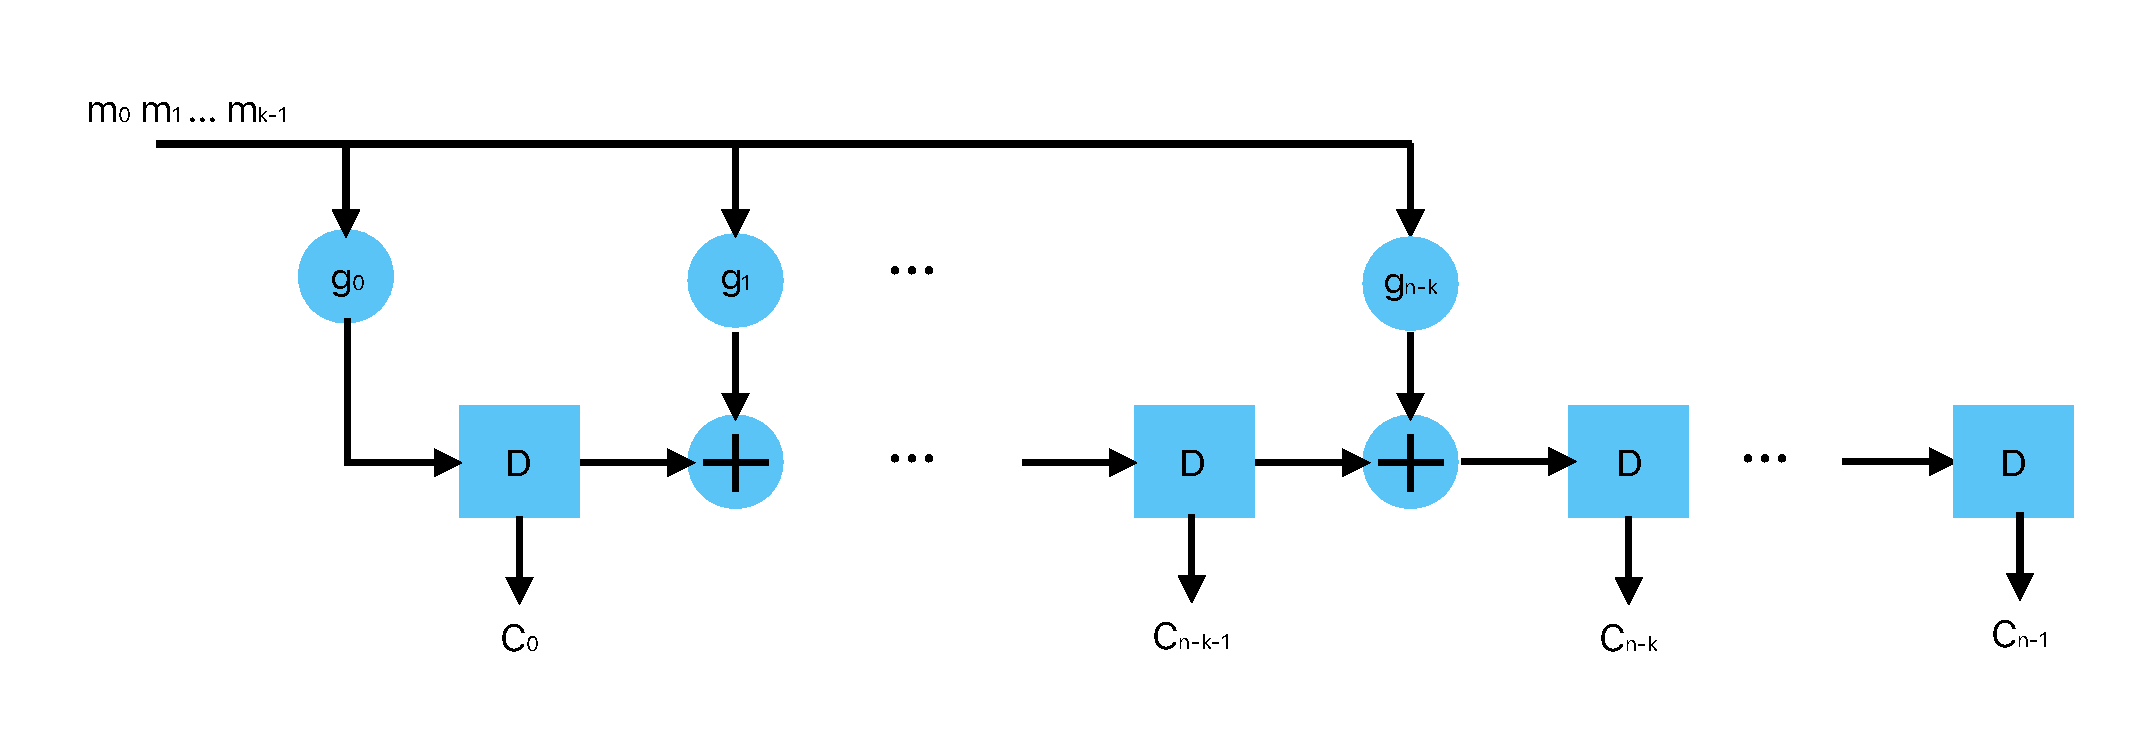
\includegraphics[width=1.0\textwidth]{Figs/CyclicCodesEncoder.pdf}
    \caption{General shift register circuit for a non-systematic encoder}
    \label{fig:CyclicEncoder}
\end{figure}

\begin{example}
Let us consider the encoding circuit for the \((7,3)\) code defined by the generator polynomial \(g(x)= x^4 + x^3 + x^2 + 1\) as in Example~\ref{ex:cyclic74}.
\begin{figure}[ht]
    \centering
    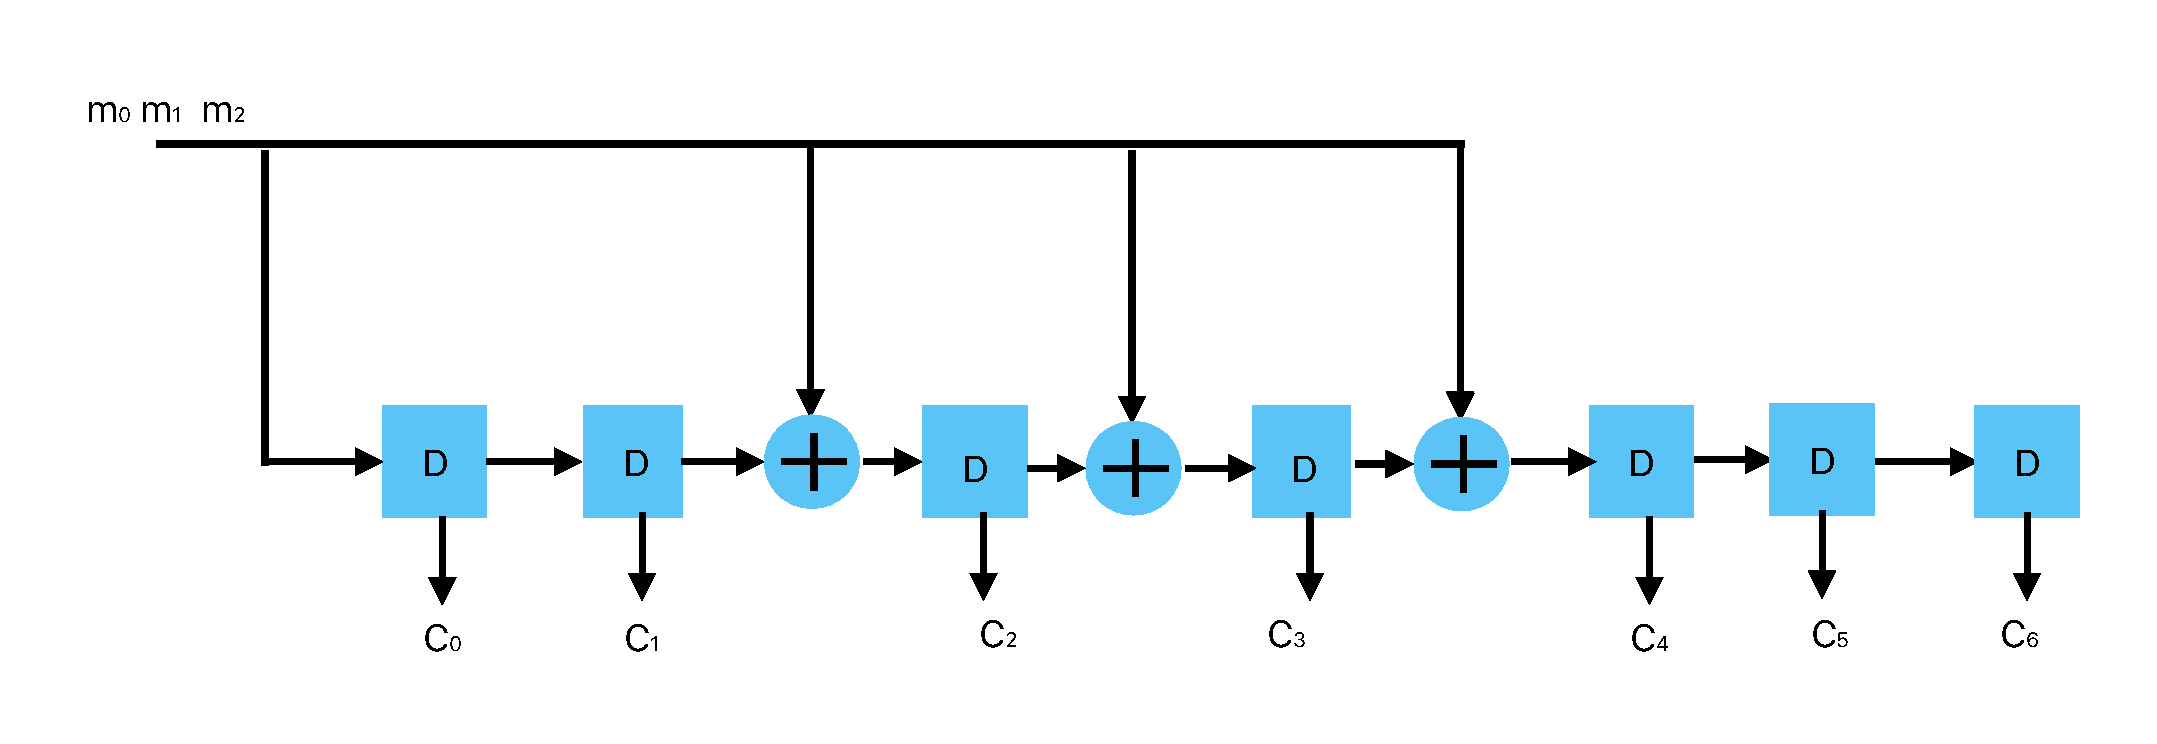
\includegraphics[width=1.0\textwidth]{Figs/SR_encoder73.pdf}
    \caption{(7,3) Encoder for the code defined in Example~\ref{ex:cyclic74} }
    \label{fig:CyclicEncoder}
\end{figure}

\end{example}


\subsection{Shift register circuit for systematic encoder}
The systematic encoding requires slightly more complicated circuit. It uses the linear-feedback shift register (LFSR) structure. The circuit computes the \(d(x) = x^{n-k} m(x) \pmod{g(x)}\). Here we will use the Example~\ref{ex:cyclic74}  to show the encoding circuits and steps. 

\begin{example}
Let us consider the systematic encoding circuit for the \((7,3)\) code defined by the generator polynomial \(g(x)= x^4 + x^3 + x^2 + 1\) as in Example~\ref{ex:cyclic74}. It has two parts: 
\begin{enumerate}
    \item The circuit for \(x^4 m(x) = x^6 + x^4 \) can be simply done by appending four zeros at the end of the input bits. We have \(m=(101)\), so the new input is \(0000101)\).   
\item Figure~\ref{fig:CyclicEncoderSystematic} shows the circuit for polynomial division of any polynomial \(p(x)\) by generator polynomial \(g(x)\). 
\end{enumerate}

\begin{figure}[ht]
    \centering
    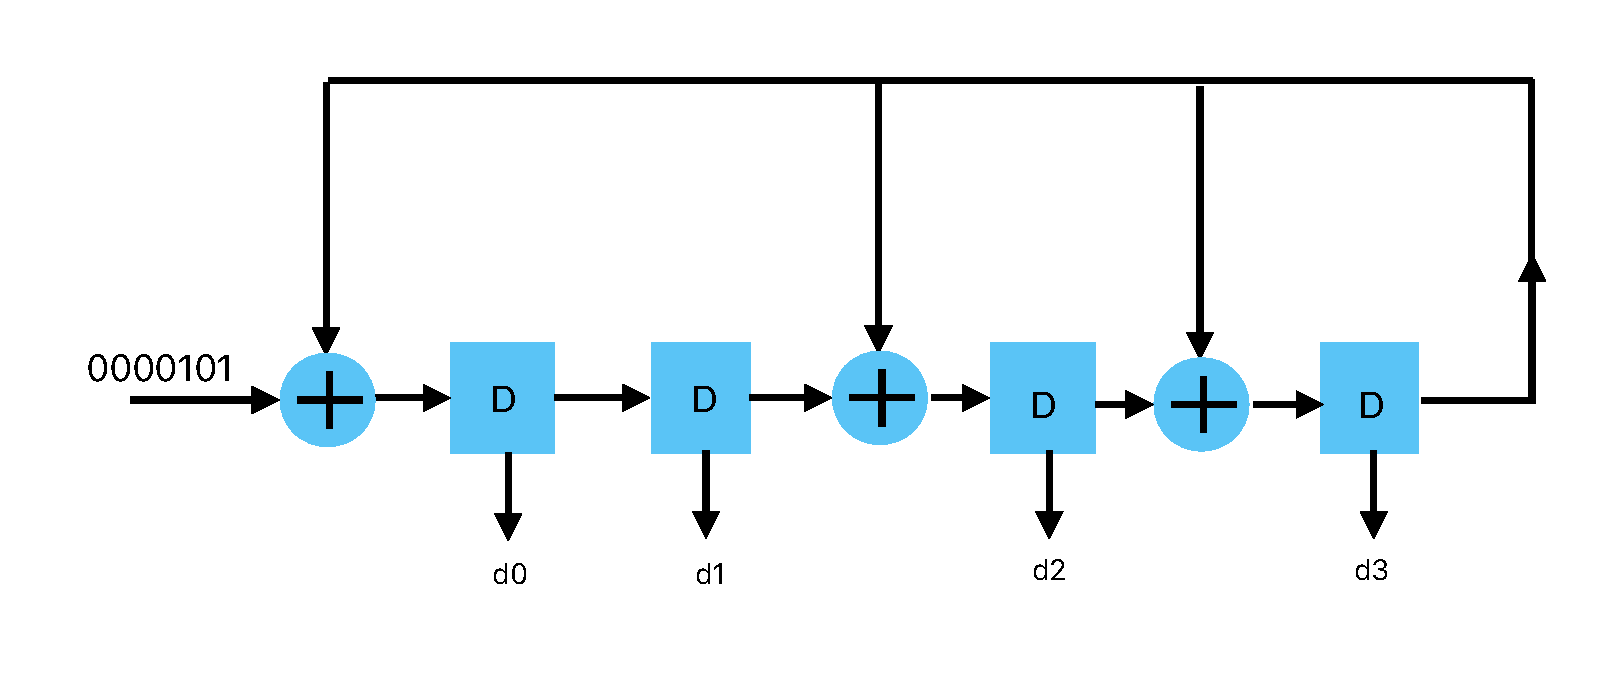
\includegraphics[width=1.0\textwidth]{Figs/SR_systematic_73.pdf}
    \caption{(7,3) Encoder for the code defined in Example~\ref{ex:cyclic74} }
    \label{fig:CyclicEncoderSystematic}
\end{figure}

The idea of the circuit is very simple; it corresponds directly to polynomial long division. The \(d(x)\) holds the current degree \(4\) polynomial as in the long division. If the leading coefficient \(d_3\) is \(1\), we subtract \(g(x)\) from the \(d(x)\); and the next \(d'(x) = x d(x)\).   

\end{example}


\section{Detection and Decoding}
Consider systematic encoding with generator polynomial \(g(x)\), we generate codeword \(c(x) = c(x)=x^{n-k}m(x) + d(x)\), where \(d(x) = x^{n-k}m(x) \pmod{g(x)} \). We will show that error detection is extremely easy and efficient, and error correction can apply syndrome decoding with a smaller look-up table. 

\subsection{Detection}
Given a received vector \(r(x)\) with systematic encoder, we can check whether it is a multiple of \(g(x)\) to detect error. A correct codeword is \(x^{n-k}m(x) + d(x)\). Assuming the input is \(m(x)\), we can use the exact encoding circuit to generate \(d(x)\). If \(r = [d', m]\) and \(d'(x) \neq d(x)\), then an error is detected.

\subsection{Decoding}
The difference \(s(x) = d'(x) - d(x) = (x^{n-k}m(x) + d'(x)) - (x^{n-k}m(x) + d(x)) = r(x) - c(x)\) is the syndrome of the received vector. Thus the syndrome \(s(x) = r(x) \pmod{g(x)}\).
